\subsection{Ca sử dụng thêm mục lưu trữ vào chuyến đi}
\vspace{0.5cm}


\noindent 
\begin{tabularx}{\linewidth}{| l | X |} 
\hline 
\textbf{Mô tả} & Người dùng có thể lưu các địa điểm, sự kiện, nhà hàng vào chuyến đi để lên lịch trình dựa trên nó. \\ 
\hline 
\textbf{Luồng cơ bản} & 1. Người dùng chọn một chuyến đi muốn thêm mục lưu. \newline
                        2. Hệ thống lây dữ liệu chi tiết của chuyến đi và hiển thị. \newline
                        3. Người dùng bấm "Thêm mục lưu". \newline
                        4. Hệ thống điều hướng sang trang thêm mục lưu và hiển thị thanh tìm kiếm. \newline
                        5. Người dùng nhập tên địa điểm, sự kiện hoặc nhà hàng muốn thêm vào chuyến đi. \newline
                        6. Hệ thống tìm kiếm và hiển thị danh sách các mục lưu phù hợp với từ khóa tìm kiếm. \newline
                        7. Người dùng chọn mục muốn lưu trong danh sách. \newline
                        8. Hệ thống thông báo đã thêm thành công. \\
               
\hline 
\textbf{Luồng thay thế} & Người dùng bấm vào mục đã lưu sẽ bỏ lưu mục đấy. \\
       
\hline 
\textbf{Tiền điều kiện} & - Người dùng đang đăng nhập và phiên đăng nhập chưa kết thúc.\newline
- Người dùng đã tạo hoặc tham gia ít nhất một chuyến đi. \newline
- Trạng thái chuyến đi khác "Đã hoàn thành" và "Hủy". \\


\hline 
\textbf{Hậu điều kiện} & - Hệ thống thêm mục lưu của chuyến đi vào cơ sở dữ liệu.\newline
                        - Người dùng có thể xem lại mục lưu đã thêm vào chuyến đi. \\

\hline 
\textbf{Yêu cầu phi chức năng} & Hệ thống thêm mục lưu dưới 1s \\ 
\hline 
\end{tabularx}



\noindent 
\begin{tabular}{| c | c |}
    \hline
    \textbf{Biểu đồ hoạt động} & \textbf{Quan hệ} \\ 
    \hline
    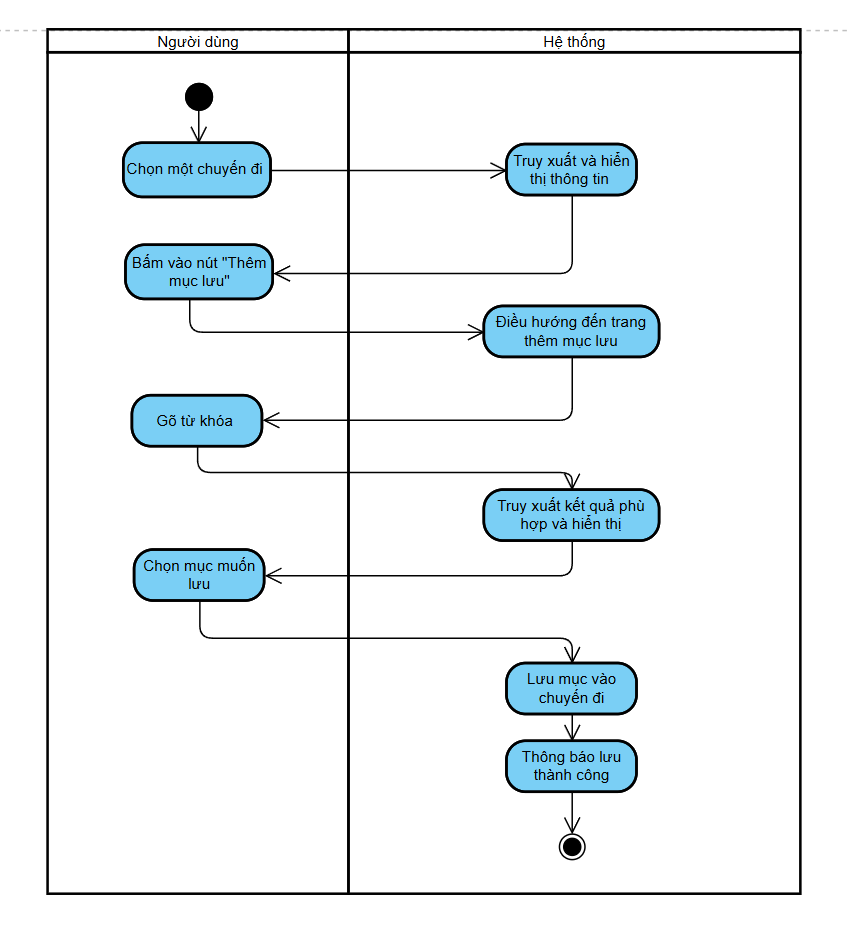
\includegraphics[width=0.5\linewidth]{figures/c3/3-3-12-ad.png} 
    & 
    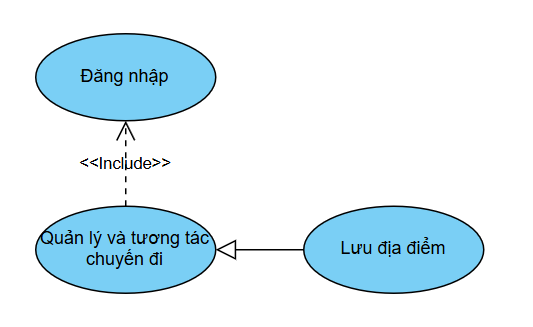
\includegraphics[width=0.45\linewidth]{figures/c3/3-3-12-rd.png} \\ 
    \hline
\end{tabular}

\vspace{0.8cm}

\begin{figure}[H]
    \centering  
    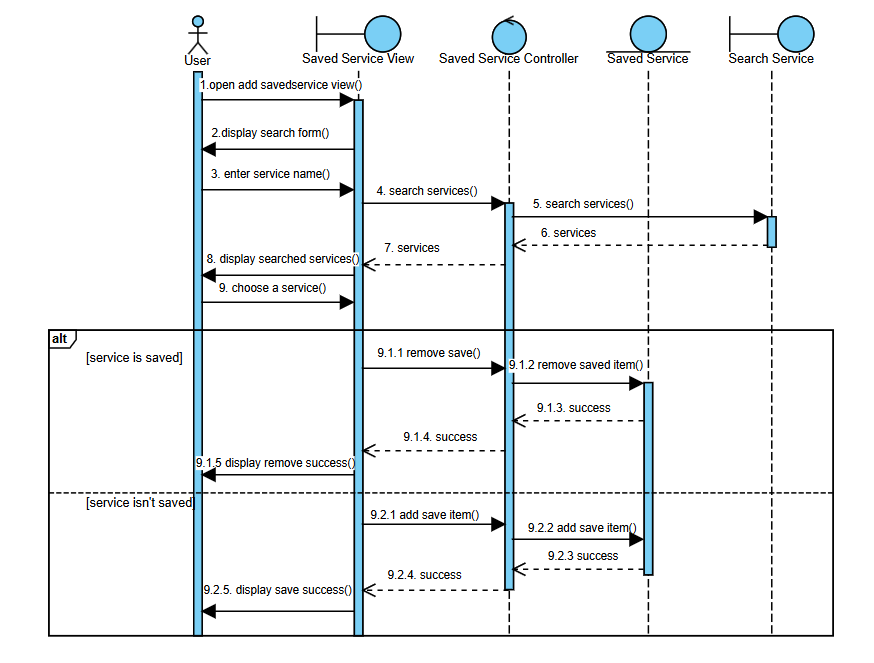
\includegraphics[width=1\textwidth]{figures/c3/3-3-12-sd.png}
    \caption{Biểu đồ tuần tự ca sử dụng thêm mục lưu vào chuyến đi.}
    \label{fig:3-3-12-sequence-diagram}
\end{figure}